\documentclass[aspectratio=169]{beamer}

% Packages
\usepackage{amsthm}        % For theorems
\usepackage{amsmath}       % For math
\usepackage{luatexja}      % For Japanese
\usepackage{booktabs}      % For formal tables
\usepackage{amssymb}       % For checkmark
\usepackage[noend]{algpseudocode}
\usepackage[backend=biber,
            style=alphabetic,
            sorting=none
            ]{biblatex}    % For bibliography
\usepackage{tikz}          % For figures
\usepackage{multirow}      % For multirow in tables
\usetikzlibrary{arrows.meta,
                chains,
                positioning}

\newcommand{\checkbox}[1]{%
  \ifnum#1=1
    \makebox[0pt][l]{\raisebox{0.15ex}{\hspace{0.1em}$\checkmark$}}%
  \fi
  $\square$%
}

\addbibresource{references.bib}

% Beamer settings
\setbeamertemplate{theorems}[numbered]
\addtobeamertemplate{theorem begin}{\normalfont}{}
\newtheorem*{sproof}{Sketch of the proof.}
\newtheorem*{remark}{Remark}
\newtheorem*{algorithm}{Algorithm}

% Theme
\usetheme{metropolis}
\usecolortheme{default}
\metroset{block=fill}

% Fonts
\setbeamerfont{title}{size=\large,series=\bfseries}
\setbeamerfont{theorem}{shape=\upshape}
\usefonttheme{professionalfonts}
\usefonttheme{structurebold}
\setbeamerfont{title}{size=\LARGE}
\setbeamerfont{date}{size=\small}
\setbeamerfont{frametitle}{size=\large,series=\bfseries}
\usepackage[T1]{fontenc}
\usepackage{mlmodern}
\usepackage{luatexja-otf}
\renewcommand{\kanjifamilydefault}{\gtdefault}
\renewcommand{\familydefault}{\sfdefault}

% Metadata
\title{1.4 最小点カバー問題}
\subtitle{近似アルゴリズム ―離散最適化問題への効果的アプローチ― pp.10--14}
\author{岡山 大輝}
\institute{兵庫県立大学大学院 情報科学研究科\textit{(ad25r010@guh.u-hyogo.ac.jp)}}
\date{April 21, 2025}

% \AtBeginSection[]
% {
%   \begin{frame}{目次}
%     \tableofcontents[currentsection]
%   \end{frame}
% }

\begin{document}

\begin{frame}
	\titlepage{}
\end{frame}

\begin{frame}{カバーについて}
	\begin{columns}
		\begin{column}{0.4\textwidth}
			\(G = (V, E)\) に対して、\\
			\alert{頂点}集合 \(U (\subseteq V)\) を考える。
			\newline

			\structure{「\(U\) は辺 \(e = (u, v)\) を\alert{カバーする}」}
			\begin{itemize}
				\item \(u \in U \lor v \in U\)
			\end{itemize}

		\end{column}
		\begin{column}{0.6\textwidth}
			\begin{figure}
				\centering
				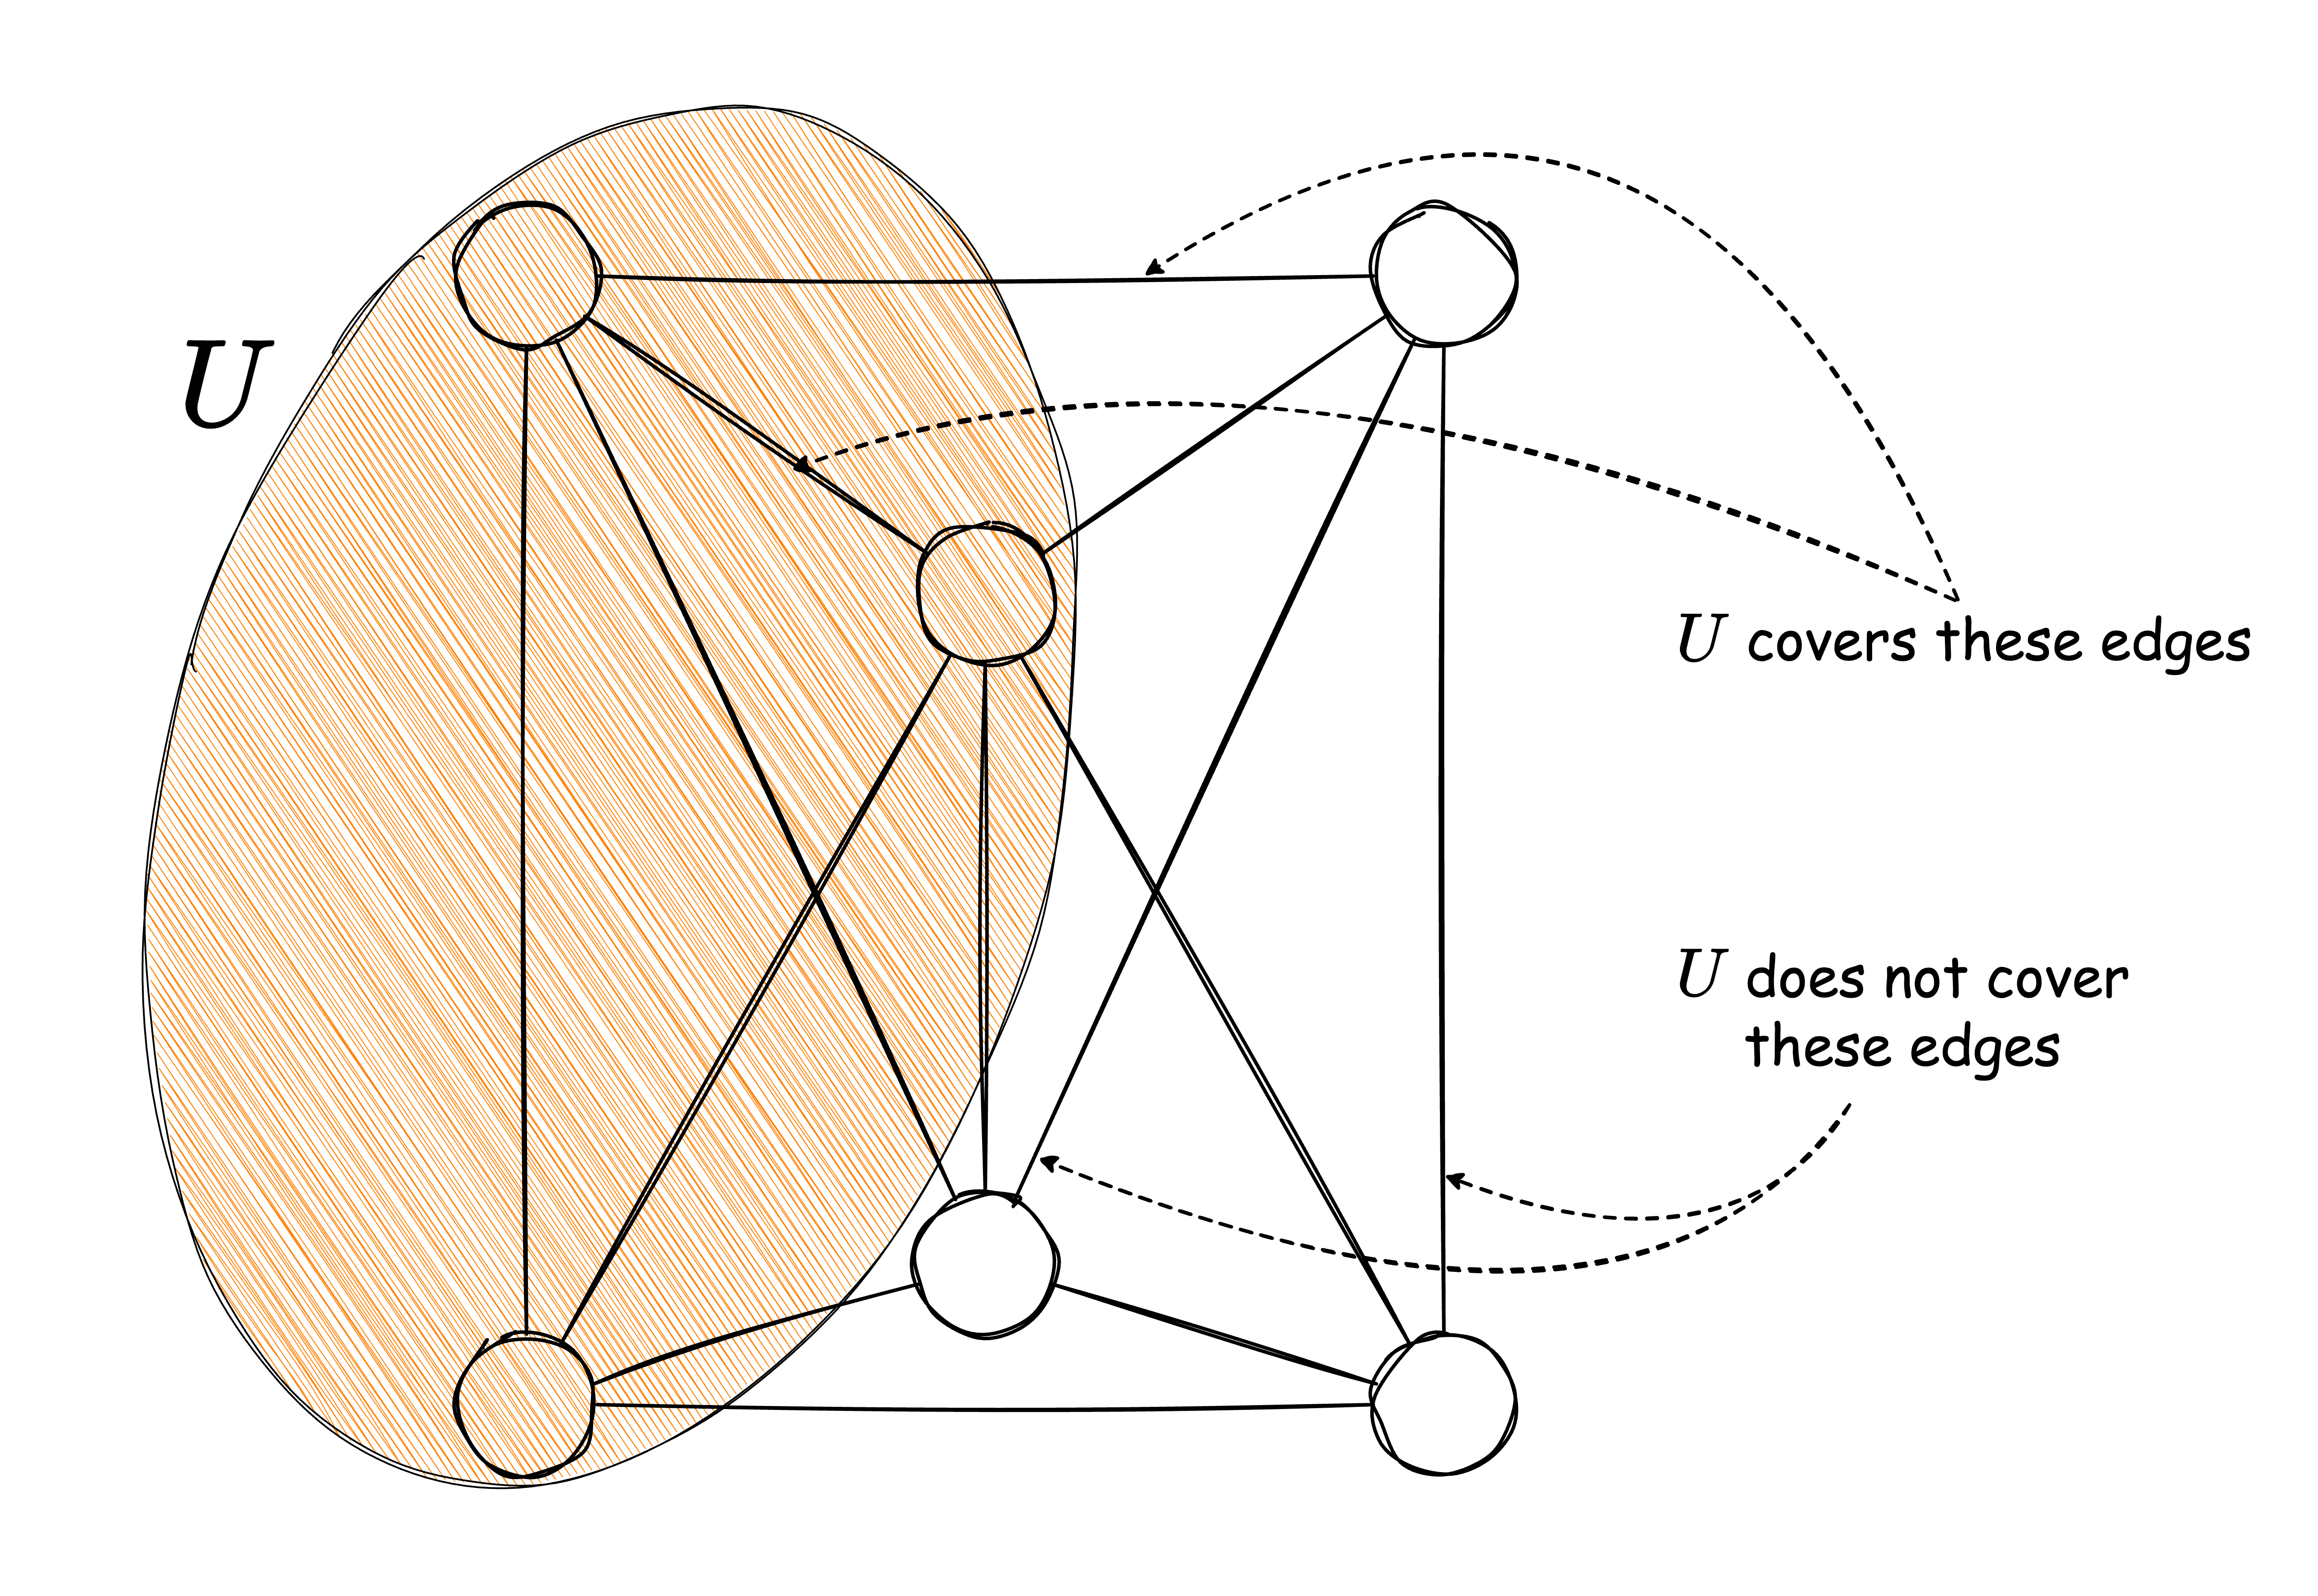
\includegraphics[width=1.0\textwidth]{figures/cover.png}
				\caption{\(U\) によってカバーされる/されない辺}
			\end{figure}
		\end{column}
	\end{columns}
\end{frame}

\begin{frame}{点カバーについて}
	\begin{columns}
		\begin{column}{0.4\textwidth}
			\structure{定義(点カバー)}
			\begin{itemize}
				\item \((u, v) \in E \Rightarrow u \in U \lor v \in U\)
			\end{itemize}
			\structure{性質}
			\begin{itemize}
				\item \(V \setminus U\) は独立集合\footnote{\(u, v \in V \setminus U \Rightarrow (u, v) \notin E\)}\footnote{\(\Rightarrow\) は明らか。では逆は??}
			\end{itemize}
		\end{column}
		\begin{column}{0.6\textwidth}
			\begin{figure}
				\centering
				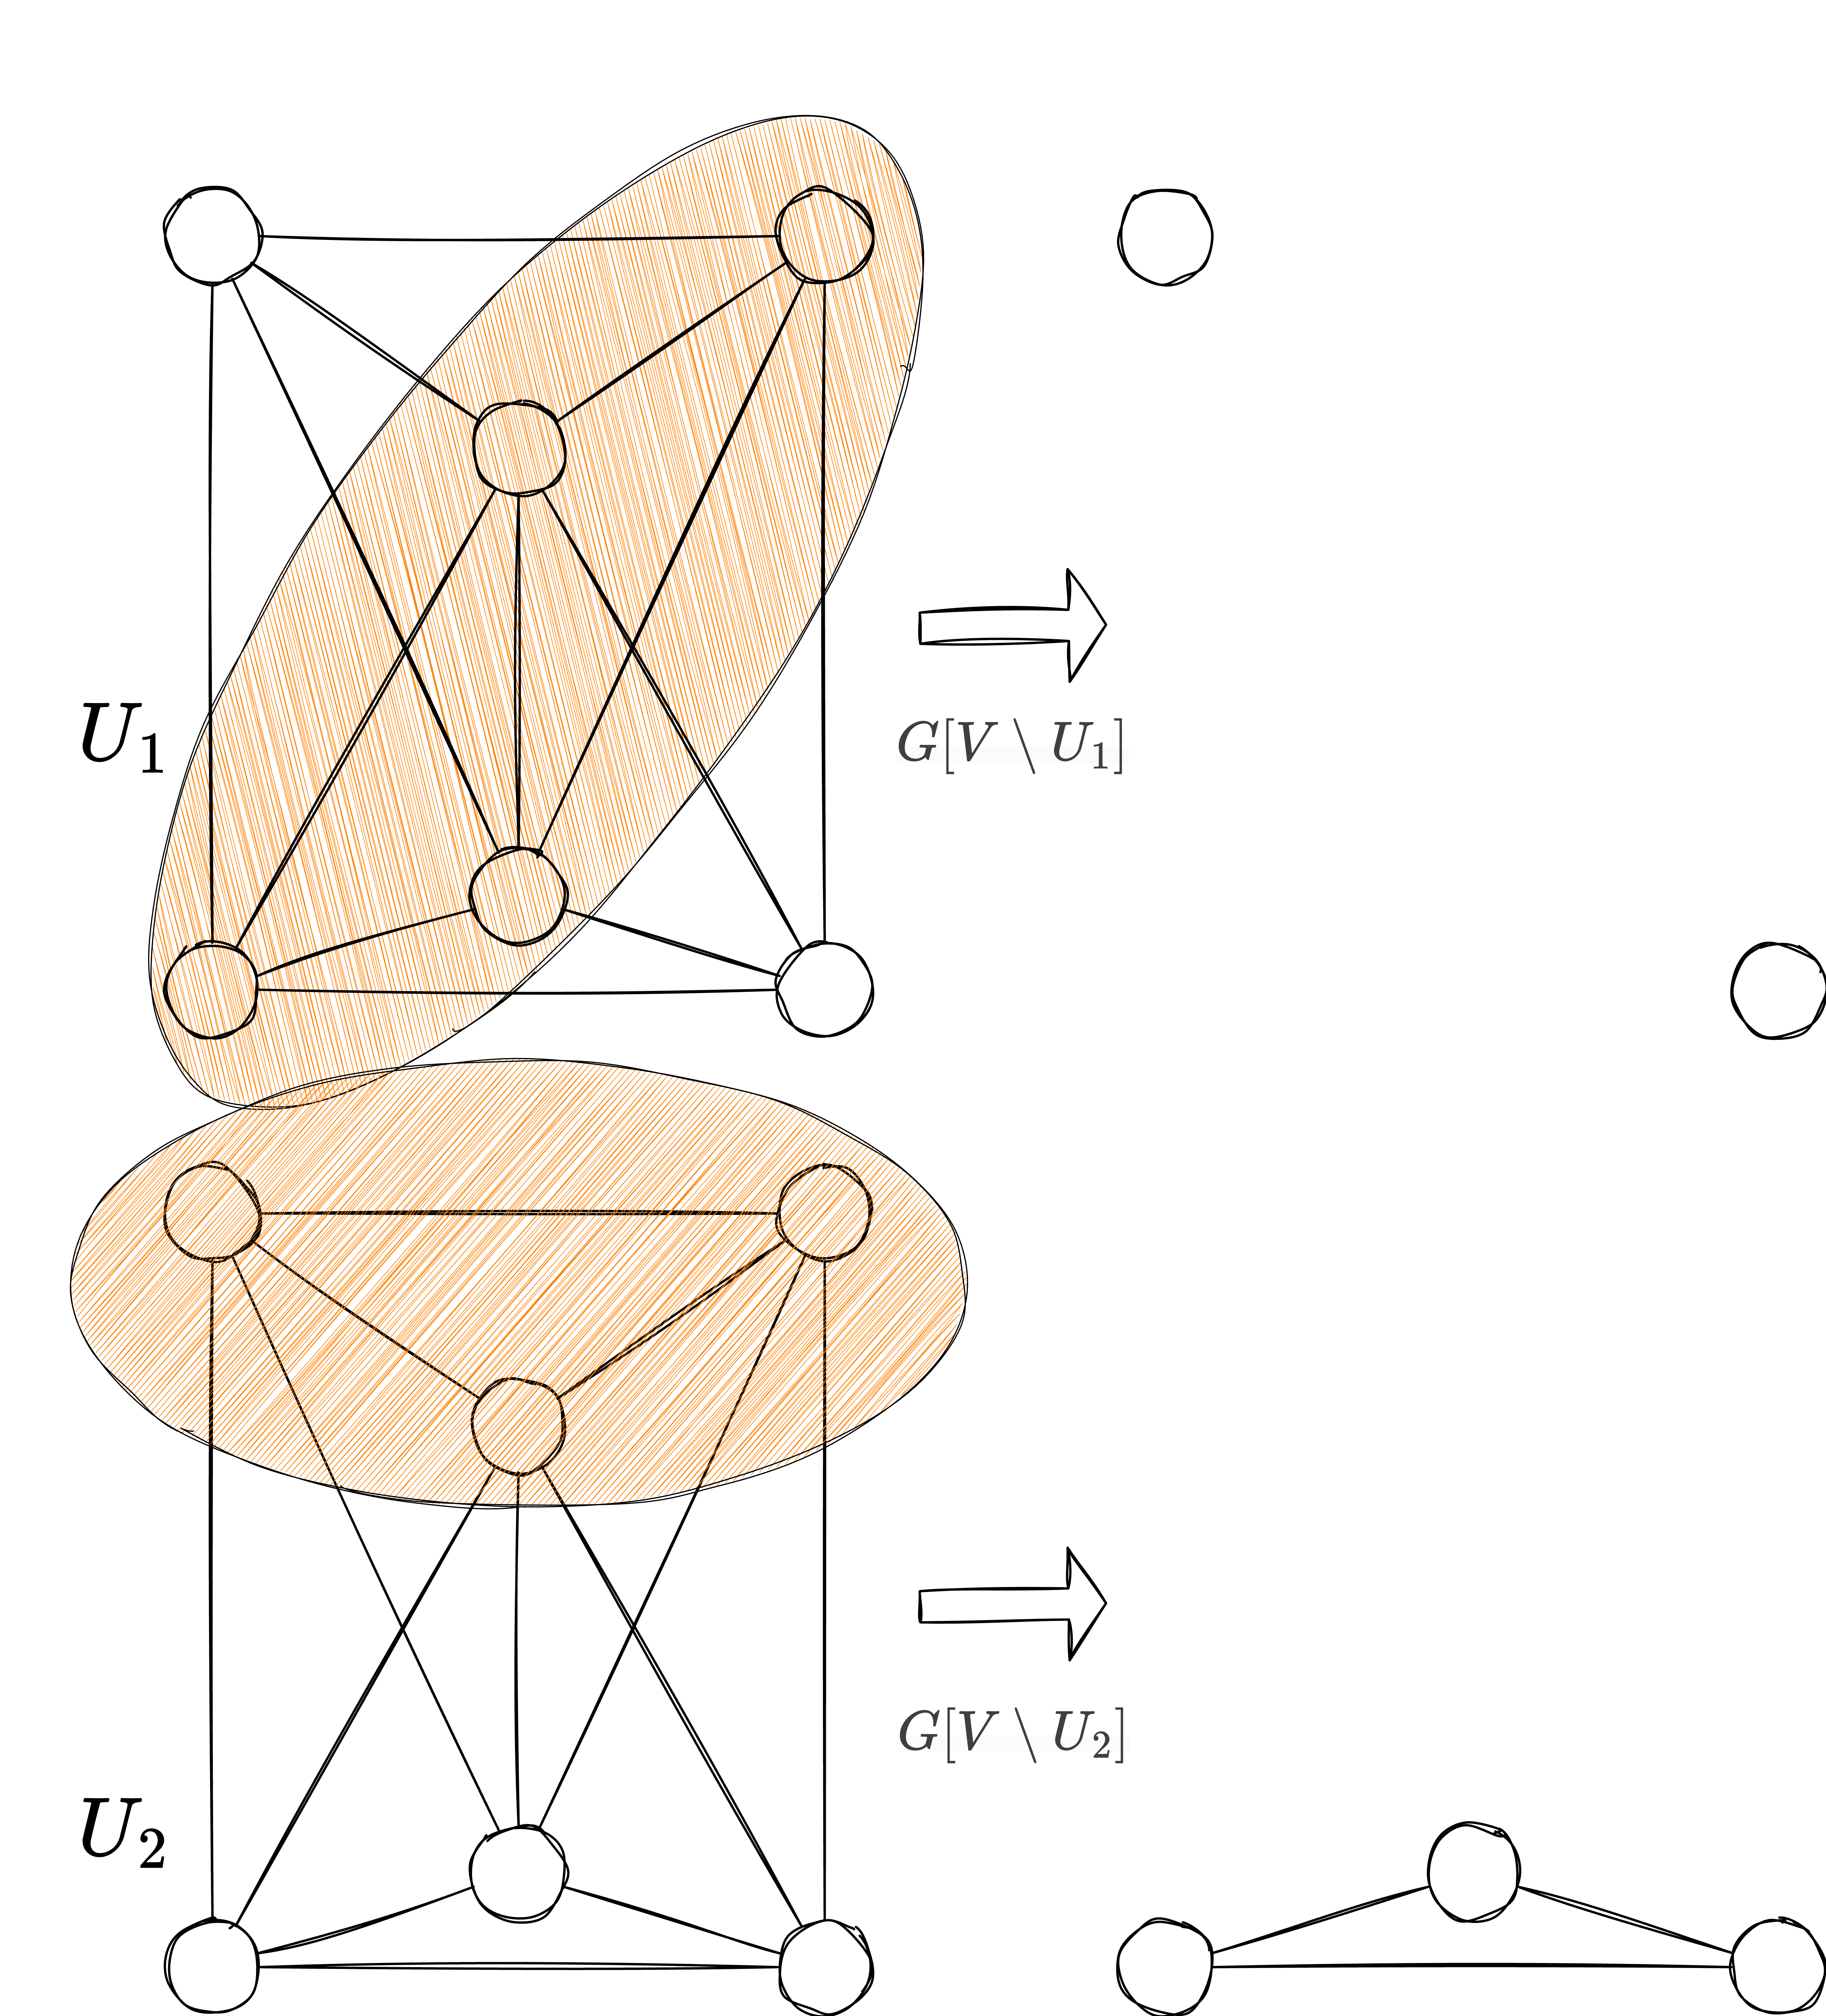
\includegraphics[width=0.65\textwidth]{figures/vertex-cover.png}
				\caption{ある点集合 \(U_1, U_2\) とそれらの補集合によって誘導されるグラフ。(\(U_1\) は点カバー、\(U_2\) は点カバーでない)}
			\end{figure}
		\end{column}
	\end{columns}
\end{frame}

\begin{frame}{最小点カバー問題と周辺の話題}
	\begin{columns}
		\begin{column}{0.5\columnwidth}
			\begin{problem}[最小点カバー問題]

			\begin{align*}
				 & \text{min.}  & |U|                                             \\
				 & \text{s.t. } & u \in U \lor v \in U &  & \forall (u, v) \in E.
			\end{align*}
			\end{problem}
		\end{column}
		\begin{column}{0.5\columnwidth}
			\begin{itemize}
				\item 最小頂点被覆問題とも
				\item $\mathcal{NP}$-困難
				      % \item $\mathcal{APX}$-完全(\(2-\epsilon\) の近似度を達成するアルゴリズムは存在しないと\alert{考えられている})
			\end{itemize}
		\end{column}
	\end{columns}
\end{frame}

% \begin{frame}{目次}
% 	\tableofcontents{}
% \end{frame}

\section{アルゴリズム}

\begin{frame}{アルゴリズムの設計の前に}
	\structure{アルゴリズムの設計と解析に対する注意 \cite{vazirani2010}}
	\begin{itemize}
		\item 近似保証を確立するために、アルゴリズムの解の値と最適解の値を比較する必要がある
		\item しかし最適解を求めることはおろか、最適値を求めることでさえ $\mathcal{NP}$-困難
	\end{itemize}

	解決策:\alert{多項式時間で計算可能な下界を最適解の値の代わりに用いる(下界スキーム)}
	\begin{figure}
		\centering
		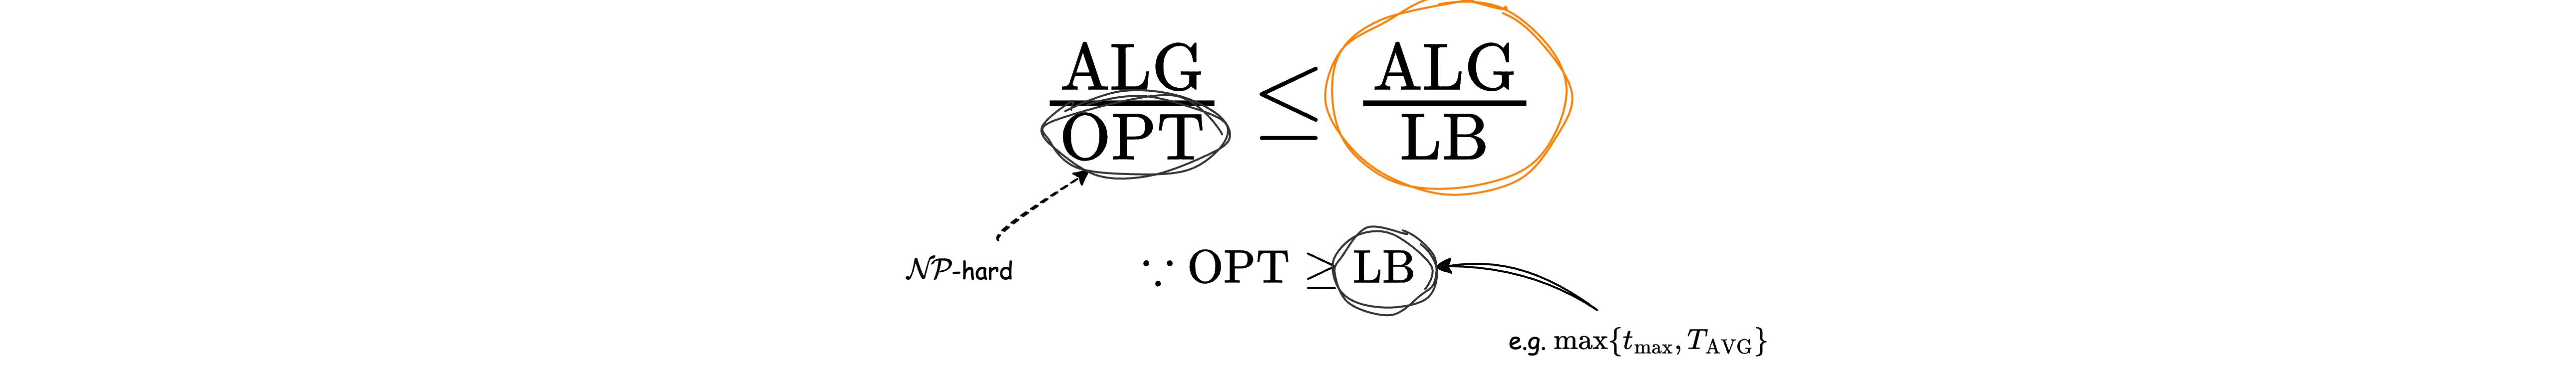
\includegraphics[width=1.4\textwidth]{figures/lower-bounding-scheme.png}
	\end{figure}
\end{frame}

\begin{frame}{準備:マッチング}
	\begin{columns}
		\begin{column}{0.5\textwidth}
			\(G = (V, E)\) に対して、\\
			\alert{辺集合} \(M (\subseteq E)\) を考える。
			\begin{itemize}
				\item \structure{「\(M\) は\alert{マッチング}である」}
				      \begin{itemize}
					      \item \(M\) のどの 2 辺も端点を共有しない
				      \end{itemize}
				\item \structure{「\(M\) は\alert{極大マッチング}である」}
				      \begin{itemize}
					      \item 集合の包含関係のもとで極大
				      \end{itemize}
				\item \structure{「\(M\) は\alert{最大マッチング}である」}
				      \begin{itemize}
					      \item 辺数最大
				      \end{itemize}
			\end{itemize}
		\end{column}
		\begin{column}{0.5\textwidth}
			\begin{figure}
				\centering
				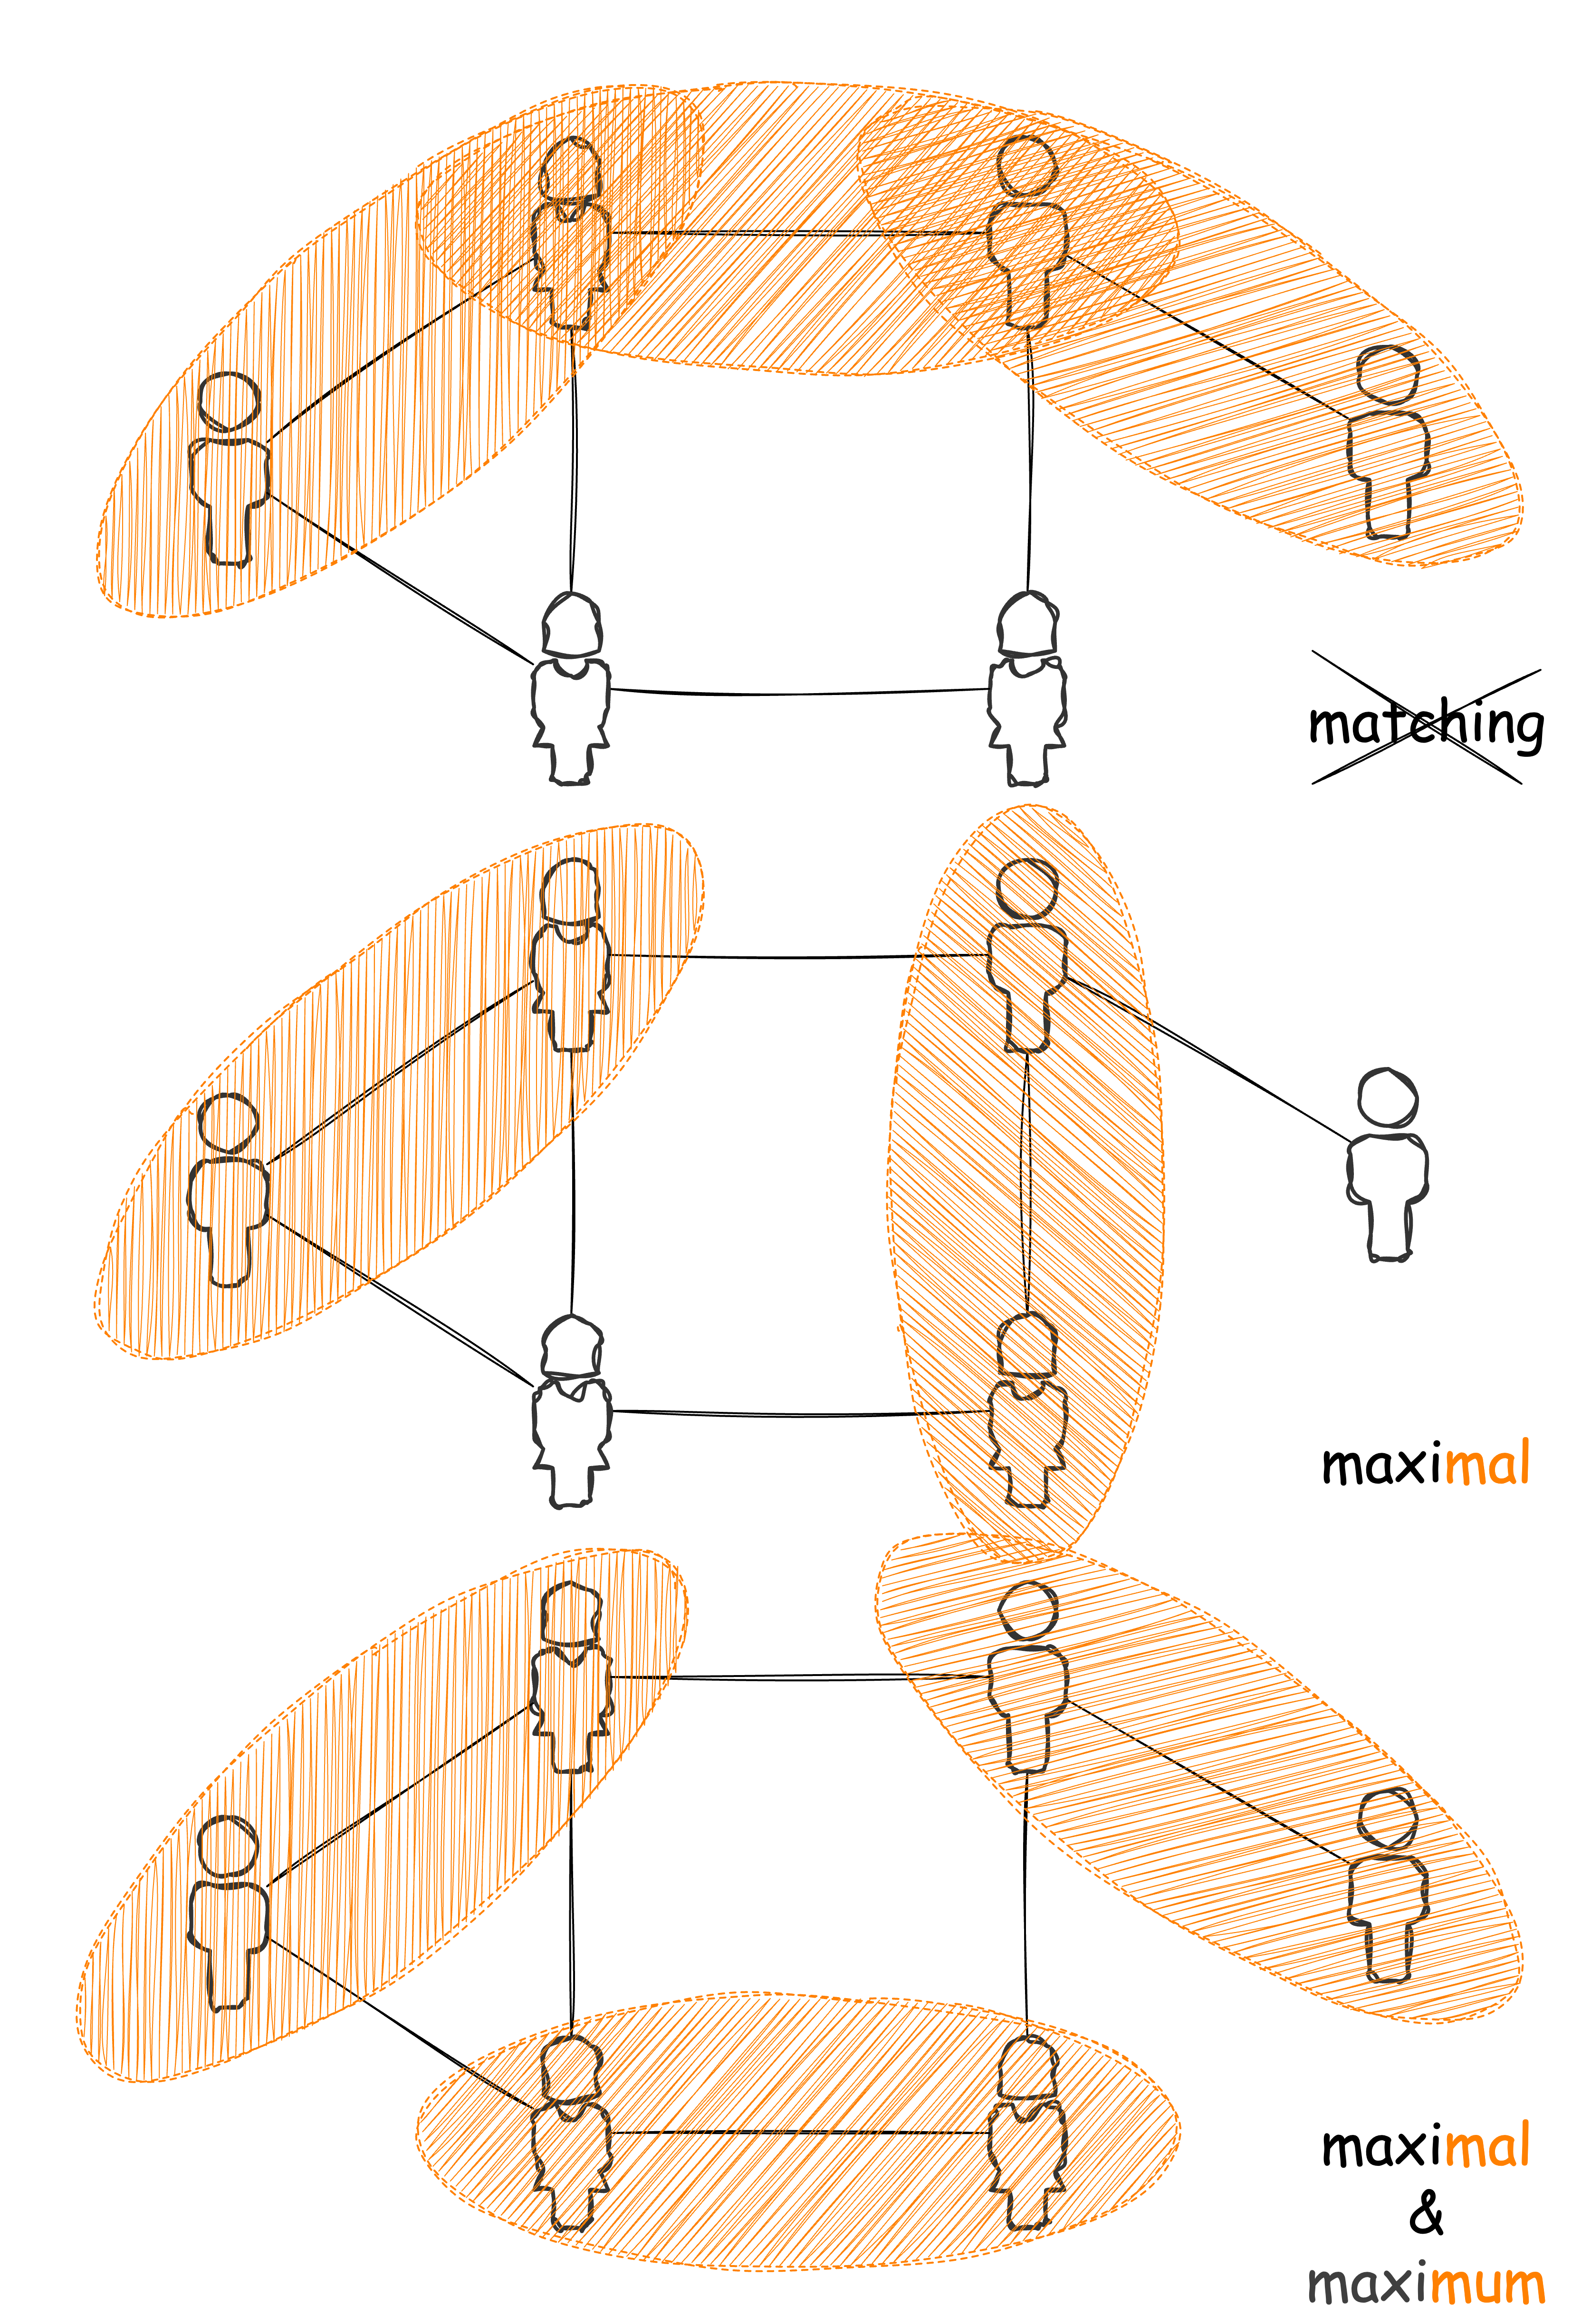
\includegraphics[width=0.65\textwidth]{figures/matching.png}
				\caption{マッチング/マッチングでない例}
			\end{figure}
		\end{column}
	\end{columns}

\end{frame}

\begin{frame}{アルゴリズム}
	\begin{algorithm}
		\(G\) の極大マッチング \(M\) を求め、\(M\) の辺の端点からなる集合を点カバーとして出力。
	\end{algorithm}

	\begin{lemma}
		アルゴリズムが出力する集合は点カバーである。
	\end{lemma}

	\begin{proof}
		仮にカバーされない辺が存在するとすると、その辺をマッチングに加えることができ、これはマッチングの極大性に矛盾する。
	\end{proof}
\end{frame}

\section{近似保証解析}

\begin{frame}{アルゴリズムの近似比}
	\begin{theorem}[アルゴリズムの近似比]
		アルゴリズムは最小点カバー問題に対して近似保証 2 を達成する。
	\end{theorem}

	\begin{proof}
		\begin{itemize}
			\item アルゴリズムが出力する点カバー \(U\) の点数は \(|U| = 2|M|\)
			\item 最小点カバー \(U^*\) の点数は \alert{\(|U^*| \ge |M|\)} (後で示す)
			\item 以上より、\[\frac{|U|}{\alert{|U^*|}} \alert{\le} \frac{2|M|}{\alert{|M|}} = 2\]
		\end{itemize}
	\end{proof}
\end{frame}

\begin{frame}{最小点カバーの下界}
	\begin{lemma}[点カバーの下界]\label{lem:lower_bound}
		任意のマッチング \(M\) と任意の点カバー \(U\) は
		\begin{equation*}
			|M| \leq |U|
		\end{equation*}
		を満たす。
	\end{lemma}

	\begin{columns}
		\begin{column}{0.47\textwidth}
			\begin{sproof}
				\begin{itemize}
					\item どの点カバーも、任意の辺の \\ 少なくとも一方の端点を含む
					\item どのマッチングの 2 辺も、\\ 端点を共有しない
				\end{itemize}
			\end{sproof}
		\end{column}
		\begin{column}{0.46\textwidth}
			\begin{figure}
				\centering
				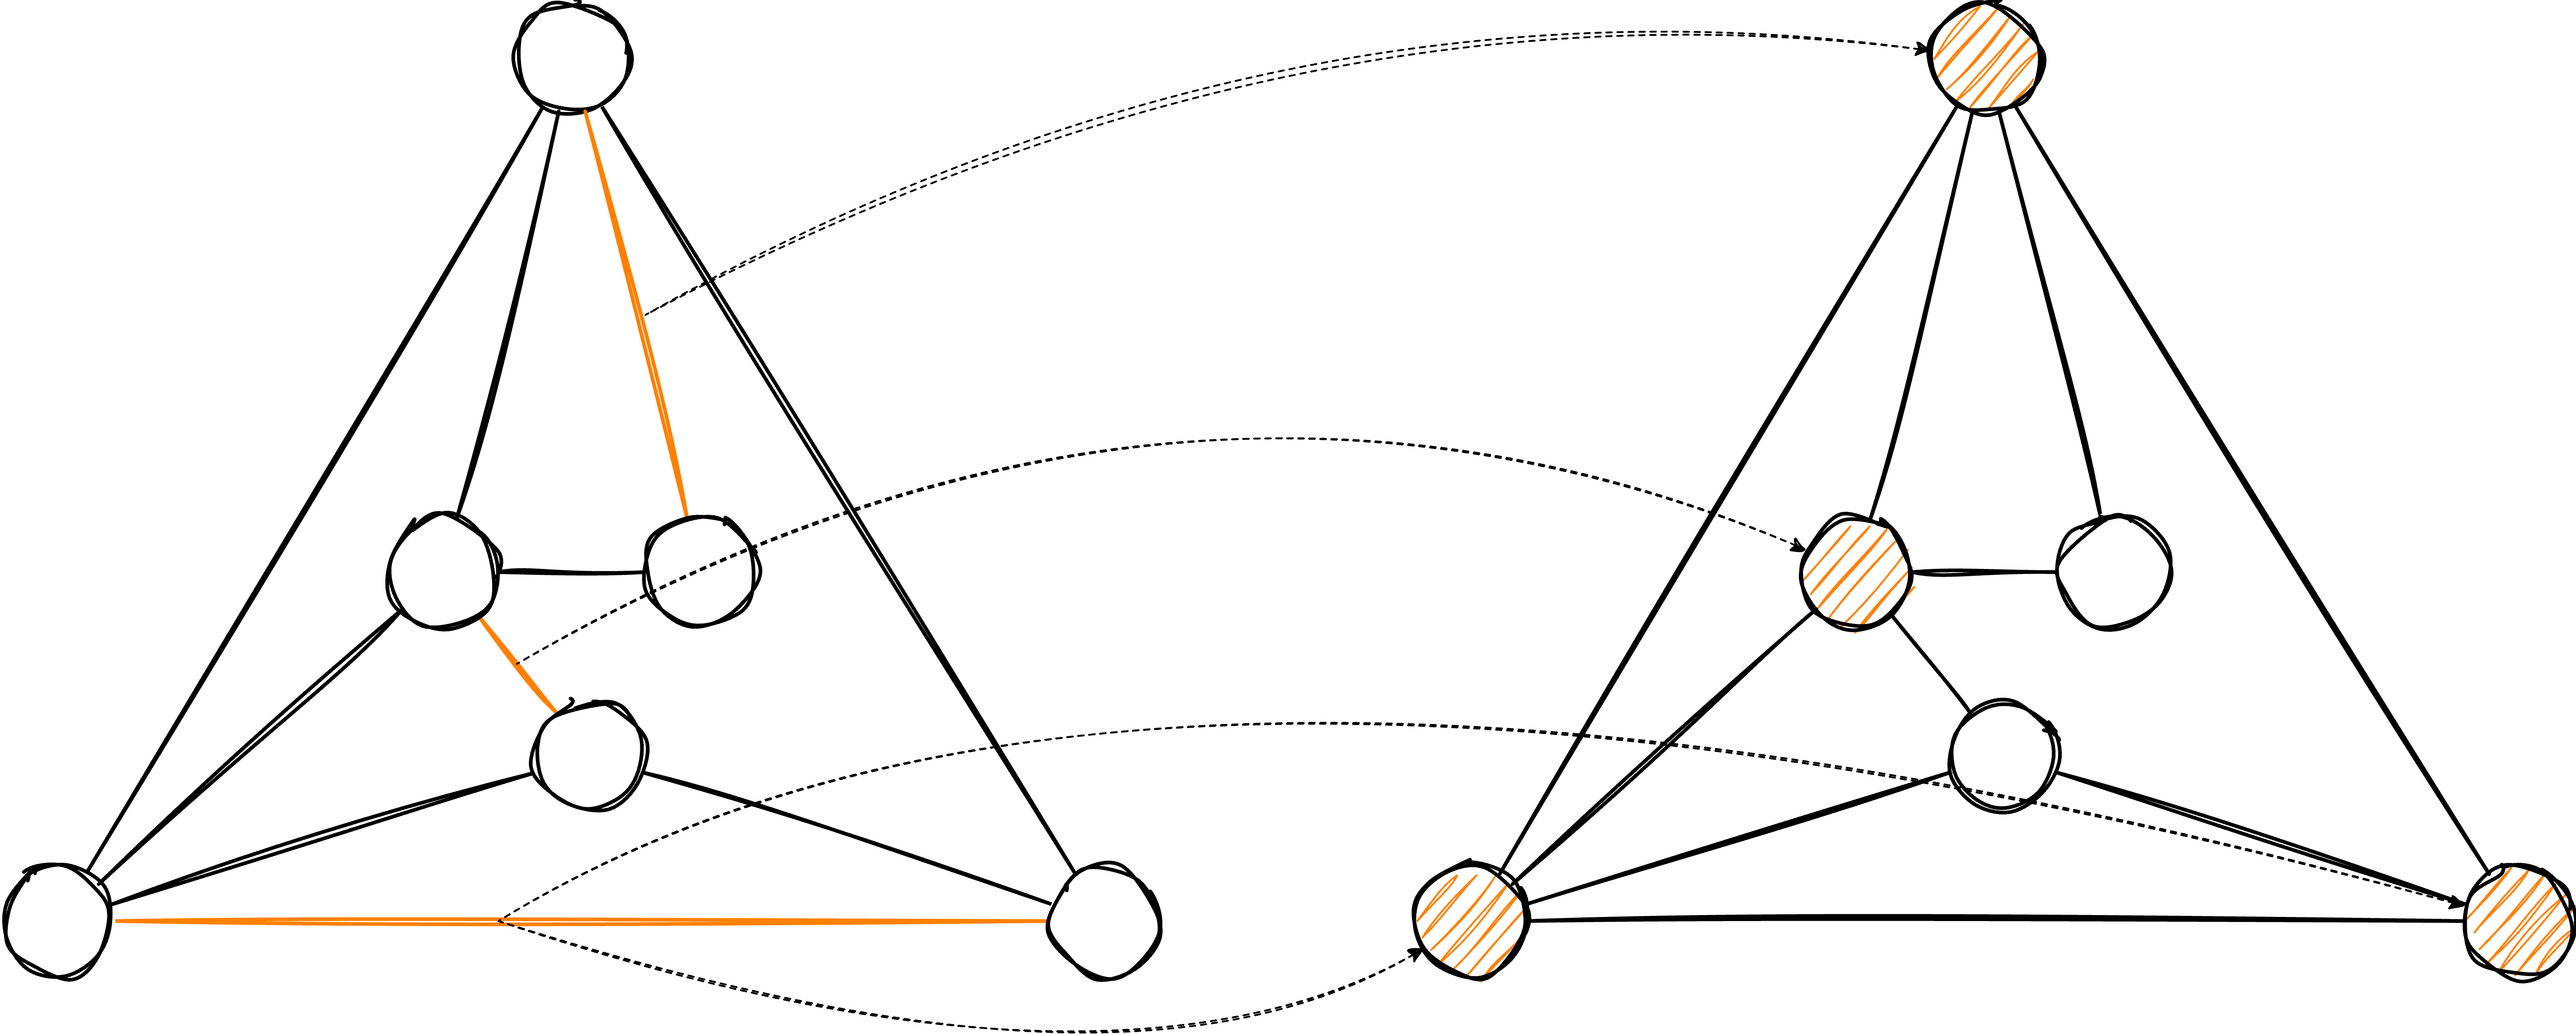
\includegraphics[width=1.0\textwidth]{figures/lower-bound.png}
				\caption{マッチングの任意の辺は、1 or 2 個の点カバーの頂点に対応付けられる}
			\end{figure}
		\end{column}
	\end{columns}
\end{frame}

\begin{frame}{[補足] アルゴリズムの時間計算量}
	\begin{remark}
		アルゴリズムの時間計算量は \(\mathcal{O}(|V| + |E|)\) である。
	\end{remark}
	\begin{itemize}
		\item すべての辺を 1 度ずつ走査する \(\mathcal{O}(|E|)\)
		\item 各辺について、端点が既にマッチングに含まれているかどうか確認する \(\mathcal{O}(1)\)
	\end{itemize}
\end{frame}

\begin{frame}{自然な疑問 \cite{vazirani2010}}
	\begin{enumerate}
		\item アルゴリズムの近似保証は解析の方法によって改善可能か?
		\item 極大マッチングの辺数を下界として用いる方法で、よりよい近似保証をもつ\\他のアルゴリズムは設計可能か?
		\item 2 未満の近似比を達成するアルゴリズムは存在するか?
	\end{enumerate}
\end{frame}

\begin{frame}{Q1. アルゴリズムの近似保証は解析の方法によって改善可能か?}
	\structure{A1. 改善できない。(近似率が 2 となる例が存在する)}

	\begin{example}[アルゴリズムの近似保証 2 のタイトな例]
		\begin{columns}
			\begin{column}{0.5\textwidth}
				完全 2 部グラフ \(K_{n, n}\) の無限個のインスタンスの族に対して、\\
				アルゴリズムが出力する解の近似率は 2 である。
			\end{column}
			\begin{column}{0.5\textwidth}
				\begin{figure}
					\centering
					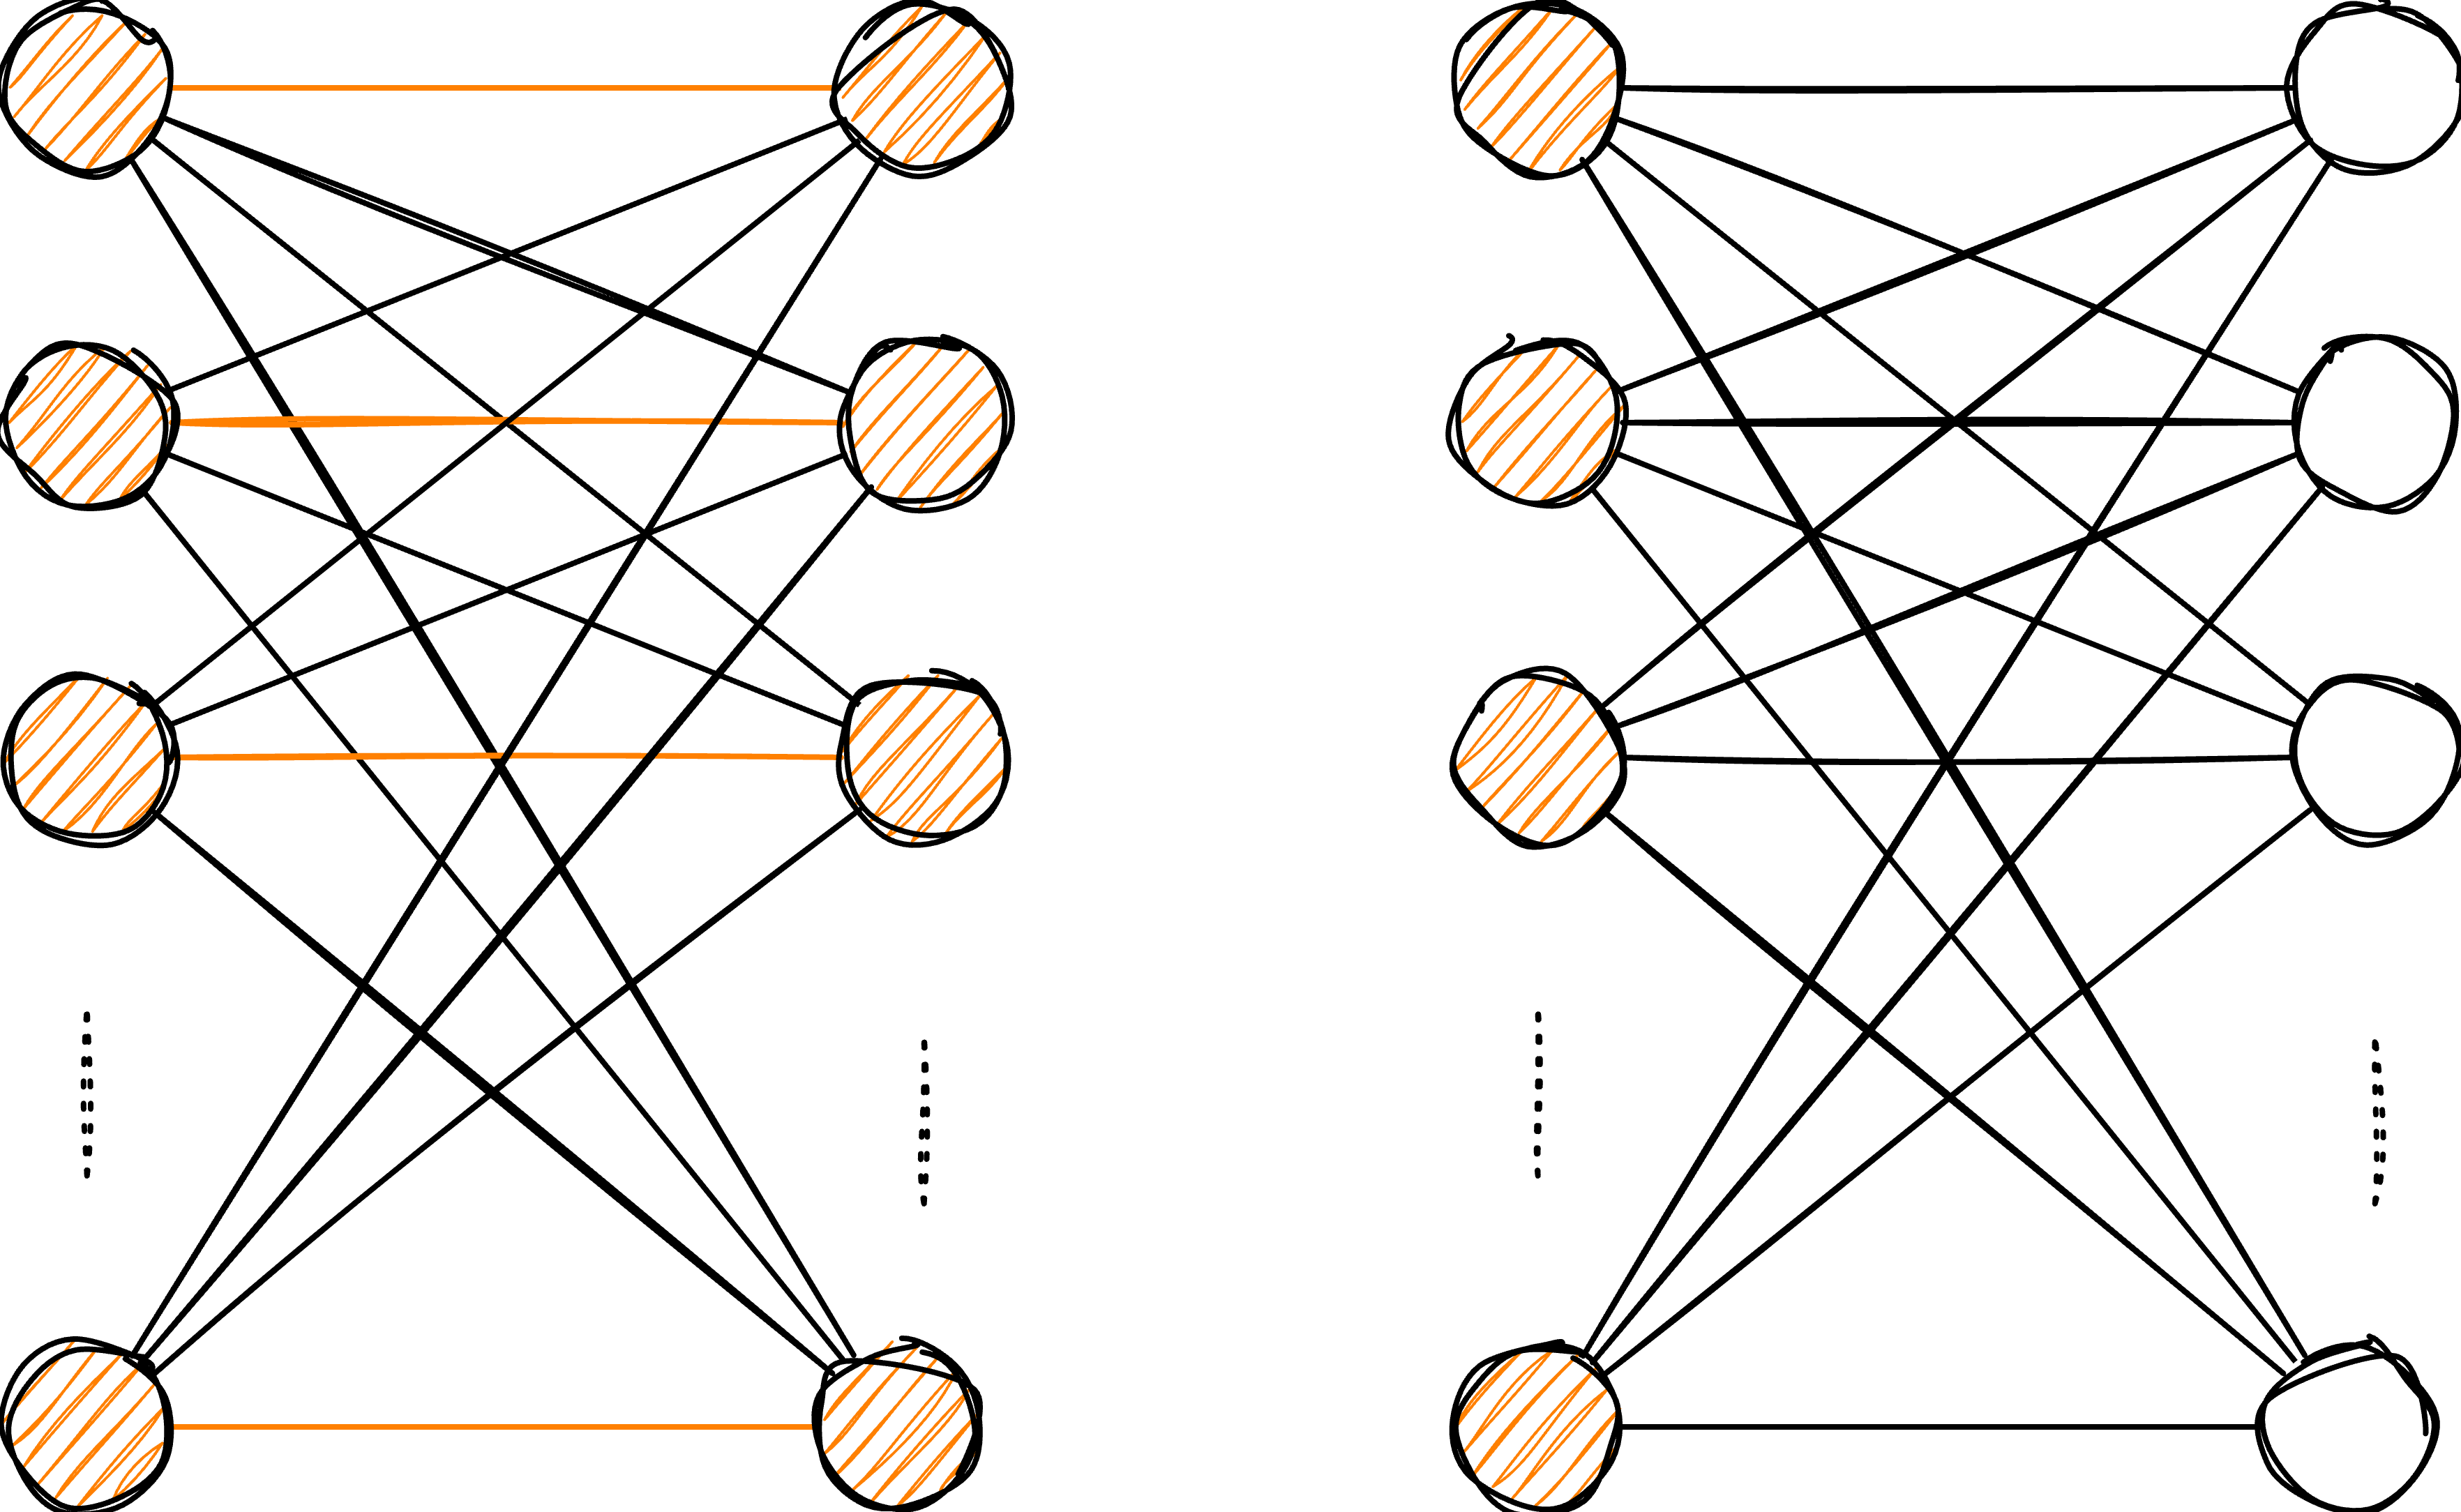
\includegraphics[width=0.8\textwidth]{figures/complete-bipertitle.png}
					\caption{完全 2 部グラフ \(K_{n, n}\) に対してアルゴリズムが出力する点カバーと最小点カバー}
				\end{figure}
			\end{column}
		\end{columns}
	\end{example}

	\alert{はたして本当にマッチング辺の両端点を追加する必要はあるのか\dots{}? (\(\Rightarrow\)Q2.)}
\end{frame}

\begin{frame}{Q2. 極大マッチングの辺数を下界として用いる方法で、よりよい近似保証をもつ\\他のアルゴリズムは設計可能か?}
	\structure{A2. 設計できない。(最適値の下界として極大マッチングを用いる限りは)}
	\begin{example}
		\begin{columns}
			\begin{column}{0.5\textwidth}
				\(n\) を奇数とすると、
				完全グラフ \(K_n\) の無限個のインスタンスの族に対して、\\
				極大マッチングの辺数は \(\frac{n-1}{2}\) であるが、\\
				最小点カバーの点数は \(n-1\) である。
			\end{column}
			\begin{column}{0.5\textwidth}
				\begin{figure}
					\centering
					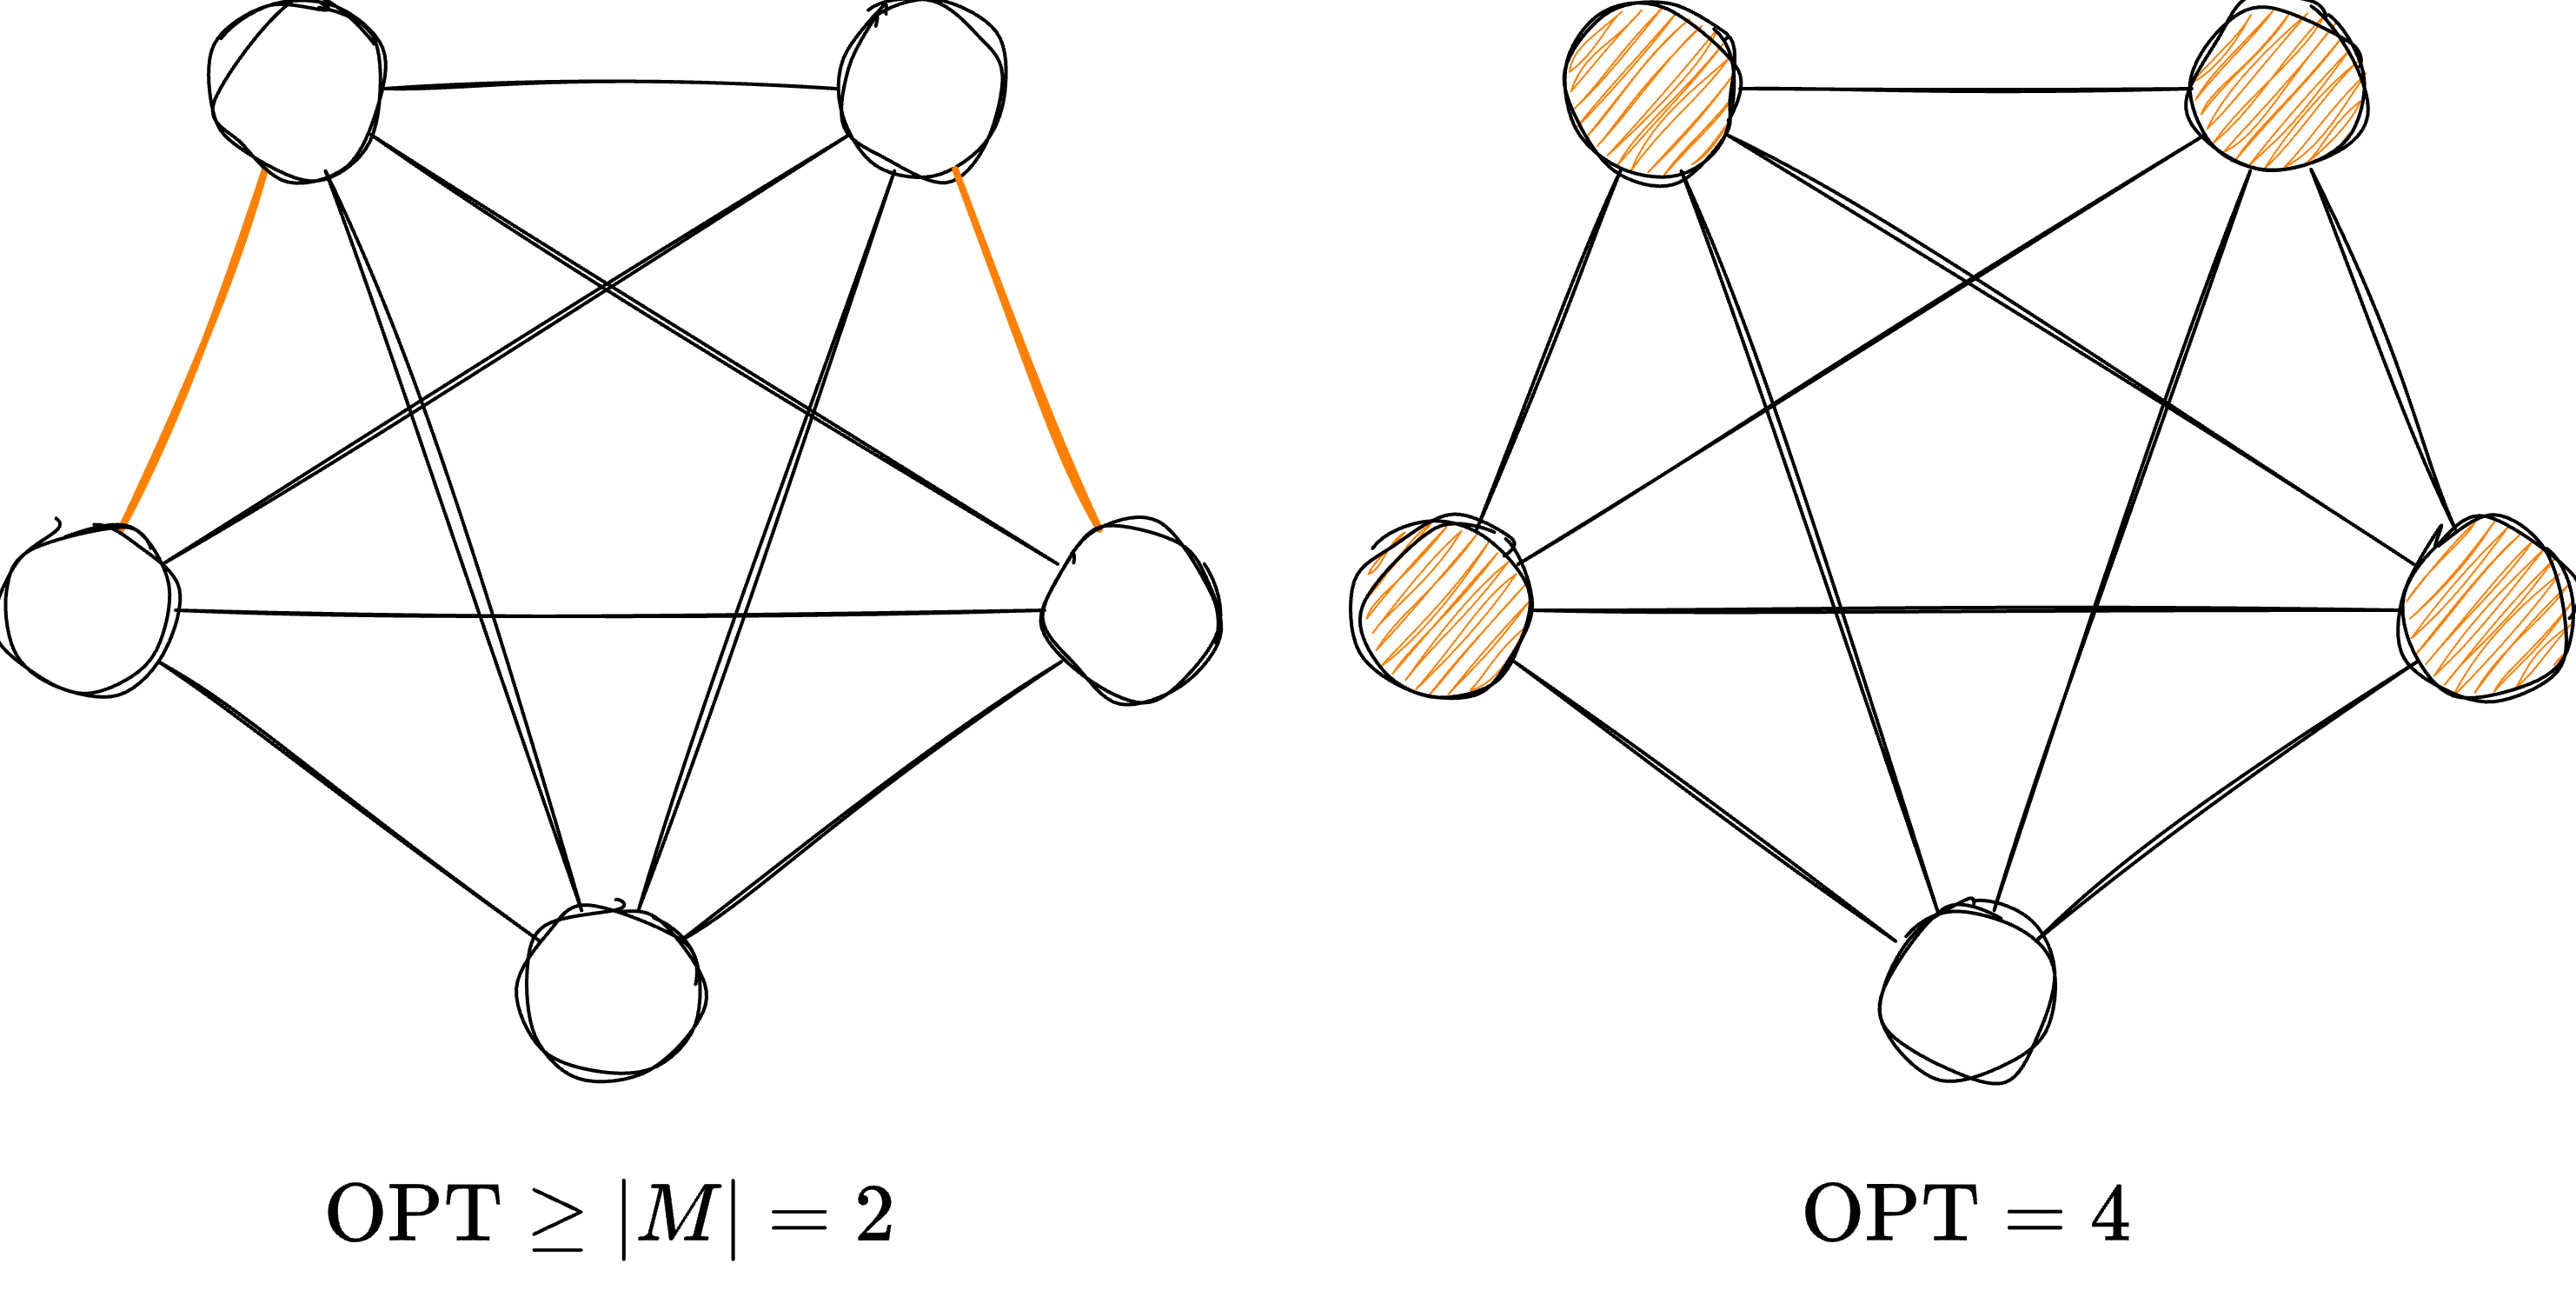
\includegraphics[width=0.9\textwidth]{figures/complete.png}
					\caption{完全グラフ \(K_5\) に対して極大マッチングから得られる最適値の下界と最小点カバー}
				\end{figure}
			\end{column}
		\end{columns}
	\end{example}

\end{frame}

\begin{frame}{Q3. 2 未満の近似比を達成するアルゴリズムは存在するか?}
	\structure{A3. 近似アルゴリズムの分野での代表的な未解決公開問題 \cite{vazirani2010}}
	\begin{itemize}
		\item 例えば、次数の高い頂点を優先的に選ぶアルゴリズムは?
	\end{itemize}
\end{frame}

\appendix

% \begin{frame}{最小点カバー問題と最大マッチング問題}
% 	\begin{quote}
% 		最小頂点被覆問題は、整数計画問題に定式化でき、その双対問題は最大マッチング問題である。\cite{wikipedia2021}
% 	\end{quote}

% 	\begin{columns}[t]
% 		\begin{column}{0.5\textwidth}
% 			\begin{align*}
% 				 & \text{min.}  & \sum_{v \in V} x_v                           \\
% 				 & \text{s.t. } & x_u + x_v \ge 1    &  & \forall (u, v) \in E \\
% 				 &              & x_v \in \{0, 1\}   &  & \forall v \in V
% 			\end{align*}
% 		\end{column}
% 		\begin{column}{0.5\textwidth}
% 			\begin{align*}
% 				 & \text{min.}  & \sum_{u,v \in E} y_{uv}                                                   \\
% 				 & \text{s.t. } & \sum_{u,v \in E : u=v' \lor v=v' } y_{uv} \le 1 &  & \forall v' \in V     \\
% 				 &              & y_{uv} \in \{0, 1\}                             &  & \forall (u, v) \in E
% 			\end{align*}
% 		\end{column}
% 	\end{columns}
% \end{frame}

% \begin{frame}{NP-completeness}

% \end{frame}

\begin{frame}[allowframebreaks]{References}
	\printbibliography{}
\end{frame}

\end{document}
